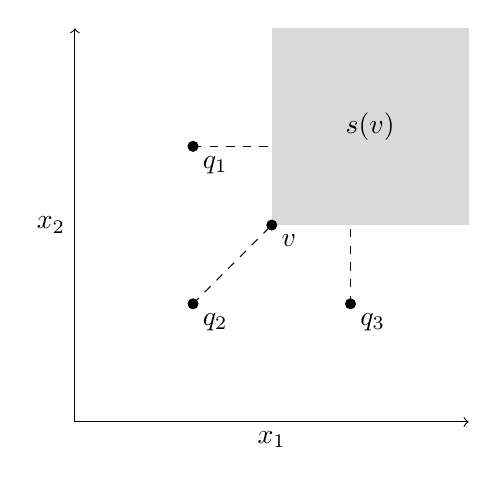
\begin{tikzpicture}
    % Draw axes
    \draw[->] (0,0) -- (5,0) node[midway, below] {\( x_1 \)};
    \draw[->] (0,0) -- (0,5) node[midway, left] {\( x_2 \)};

    % Shade the non-dominated area (above and right of v)
    \fill[gray!30] 
        (2.5,2.5) -- (2.5,5) -- (5,5) -- (5,2.5) -- cycle;
    \node at (3.75,3.75) {\( s(v) \)};
    
    % Draw the point v
    \fill (2.5,2.5) circle (2pt) node[below right] {\( v \)};
    

    % Additional points q1, q2, q3
    \fill (1.5,3.5) circle (2pt) node[below right] {\( q_1 \)};
    \fill (1.5,1.5) circle (2pt) node[below right] {\( q_2 \)};
    \fill (3.5,1.5) circle (2pt) node[below right] {\( q_3 \)};
    
    % Draw lines to the nearest boundary of the non-dominated region
    \draw[dashed] (1.5,3.5) -- (2.5,3.5);  % q1 to shaded region (horizontally right)
    \draw[dashed] (1.5,1.5) -- (2.5,2.5);  % q2 to v (diagonal)
    \draw[dashed] (3.5,1.5) -- (3.5,2.5);  % q3 to shaded region (vertically up)

\end{tikzpicture}
